\documentclass{standalone}
\usepackage{tikz}
\usetikzlibrary{patterns, positioning}

\begin{document}
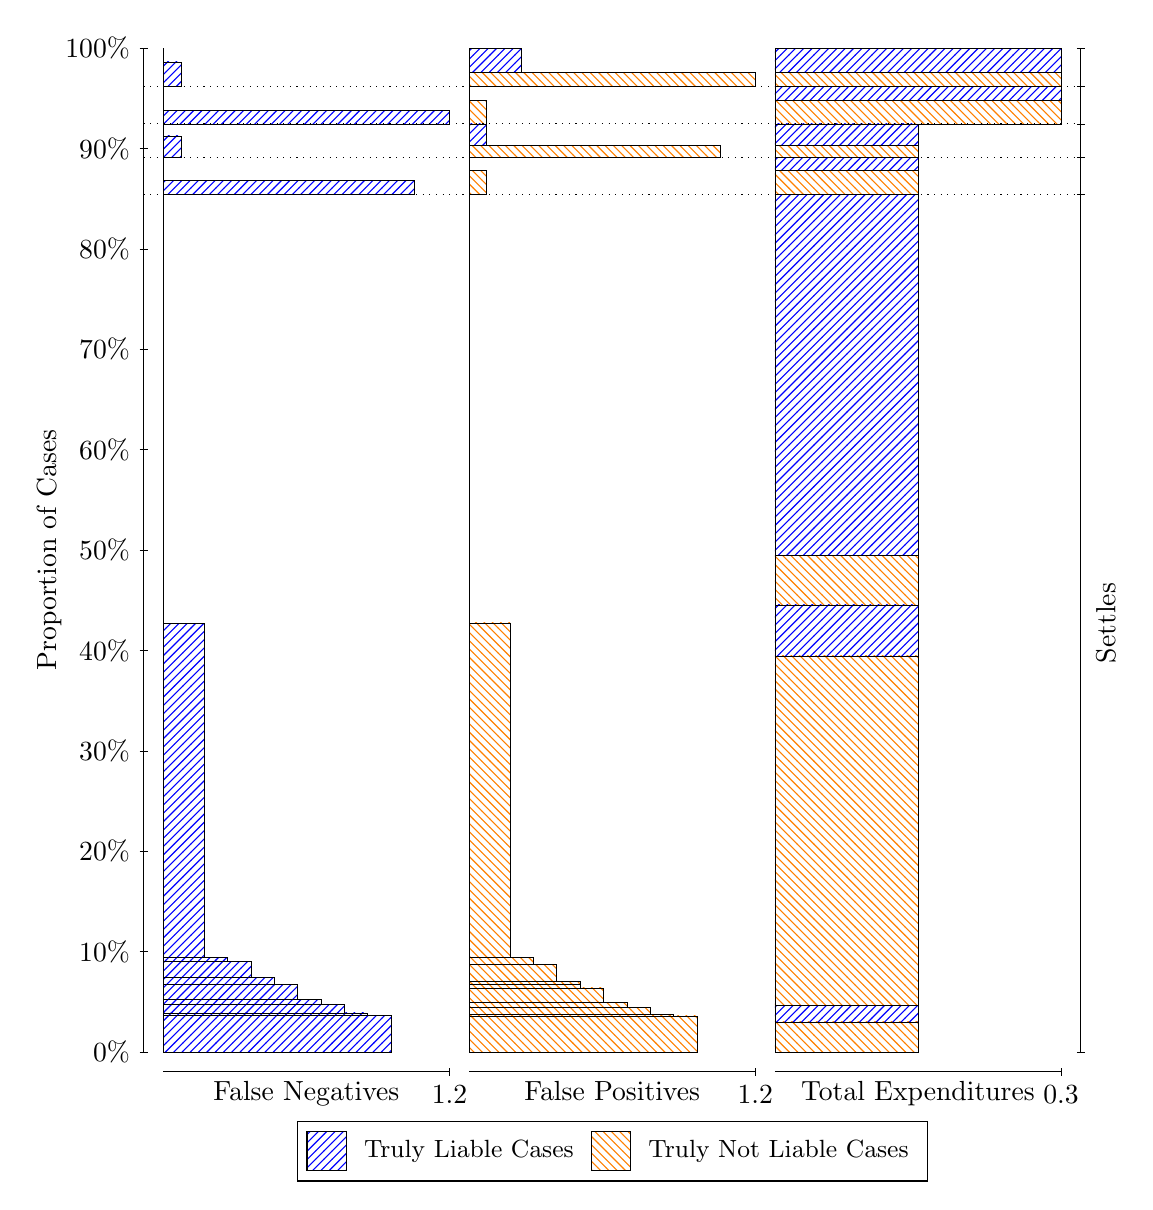
\begin{tikzpicture}
\draw[black, very thin] (1.5,1.75) -- (1.5,14.5);
\node[rotate=90, anchor=center] at (0.3, 8.125) {Proportion of Cases};
\draw[black, very thin] (1.45,1.75) -- (1.55,1.75);
\node[anchor=east] at (1.45, 1.75) {0\%};
\draw[black, very thin] (1.45,3.025) -- (1.55,3.025);
\node[anchor=east] at (1.45, 3.025) {10\%};
\draw[black, very thin] (1.45,4.3) -- (1.55,4.3);
\node[anchor=east] at (1.45, 4.3) {20\%};
\draw[black, very thin] (1.45,5.575) -- (1.55,5.575);
\node[anchor=east] at (1.45, 5.575) {30\%};
\draw[black, very thin] (1.45,6.85) -- (1.55,6.85);
\node[anchor=east] at (1.45, 6.85) {40\%};
\draw[black, very thin] (1.45,8.125) -- (1.55,8.125);
\node[anchor=east] at (1.45, 8.125) {50\%};
\draw[black, very thin] (1.45,9.4) -- (1.55,9.4);
\node[anchor=east] at (1.45, 9.4) {60\%};
\draw[black, very thin] (1.45,10.675) -- (1.55,10.675);
\node[anchor=east] at (1.45, 10.675) {70\%};
\draw[black, very thin] (1.45,11.95) -- (1.55,11.95);
\node[anchor=east] at (1.45, 11.95) {80\%};
\draw[black, very thin] (1.45,13.225) -- (1.55,13.225);
\node[anchor=east] at (1.45, 13.225) {90\%};
\draw[black, very thin] (1.45,14.5) -- (1.55,14.5);
\node[anchor=east] at (1.45, 14.5) {100\%};

\draw[black, very thin] (13.4,1.75) -- (13.4,14.5);
\draw[black, very thin] (13.35,1.75) -- (13.45,1.75);
\node[anchor=west] at (13.35, 1.75) {};
\draw[black, very thin] (13.35,12.645) -- (13.45,12.645);
\node[anchor=west] at (13.35, 12.645) {};
\draw[black, very thin] (13.35,13.115) -- (13.45,13.115);
\node[anchor=west] at (13.35, 13.115) {};
\draw[black, very thin] (13.35,13.537) -- (13.45,13.537);
\node[anchor=west] at (13.35, 13.537) {};
\draw[black, very thin] (13.35,14.011) -- (13.45,14.011);
\node[anchor=west] at (13.35, 14.011) {};
\draw[black, very thin] (13.35,14.5) -- (13.45,14.5);
\node[anchor=west] at (13.35, 14.5) {};

\draw[black, very thin, pattern color=blue, pattern=north east lines] (1.75,1.75) rectangle (4.6418,2.2098);
\draw[black, very thin, pattern color=blue, pattern=north east lines] (1.75,2.2098) rectangle (4.3452,2.2456);
\draw[black, very thin, pattern color=blue, pattern=north east lines] (1.75,2.2456) rectangle (4.0486,2.353);
\draw[black, very thin, pattern color=blue, pattern=north east lines] (1.75,2.353) rectangle (3.752,2.4199);
\draw[black, very thin, pattern color=blue, pattern=north east lines] (1.75,2.4199) rectangle (3.4554,2.6062);
\draw[black, very thin, pattern color=blue, pattern=north east lines] (1.75,2.6062) rectangle (3.1588,2.7019);
\draw[black, very thin, pattern color=blue, pattern=north east lines] (1.75,2.7019) rectangle (2.8622,2.9047);
\draw[black, very thin, pattern color=blue, pattern=north east lines] (1.75,2.9047) rectangle (2.5656,2.9475);
\draw[black, very thin, pattern color=blue, pattern=north east lines] (1.75,2.9475) rectangle (2.269,7.1961);
\draw[black, very thin, pattern color=orange, pattern=north west lines] (1.75,7.1961) rectangle (1.75,12.645);
\draw[black, very thin, pattern color=blue, pattern=north east lines] (1.75,12.645) rectangle (4.9384,12.818);
\draw[black, very thin, pattern color=orange, pattern=north west lines] (1.75,12.818) rectangle (1.75,13.115);
\draw[black, very thin, pattern color=blue, pattern=north east lines] (1.75,13.115) rectangle (1.9724,13.384);
\draw[black, very thin, pattern color=orange, pattern=north west lines] (1.75,13.384) rectangle (1.75,13.537);
\draw[black, very thin, pattern color=blue, pattern=north east lines] (1.75,13.537) rectangle (5.3833,13.711);
\draw[black, very thin, pattern color=orange, pattern=north west lines] (1.75,13.711) rectangle (1.75,14.011);
\draw[black, very thin, pattern color=blue, pattern=north east lines] (1.75,14.011) rectangle (1.9724,14.323);
\draw[black, very thin, pattern color=orange, pattern=north west lines] (1.75,14.323) rectangle (1.75,14.5);
\draw[black, very thin, pattern color=orange, pattern=north west lines] (5.6333,1.75) rectangle (8.5252,2.2091);
\draw[black, very thin, pattern color=orange, pattern=north west lines] (5.6333,2.2091) rectangle (8.2286,2.2281);
\draw[black, very thin, pattern color=orange, pattern=north west lines] (5.6333,2.2281) rectangle (7.932,2.3211);
\draw[black, very thin, pattern color=orange, pattern=north west lines] (5.6333,2.3211) rectangle (7.6354,2.3783);
\draw[black, very thin, pattern color=orange, pattern=north west lines] (5.6333,2.3783) rectangle (7.3388,2.5643);
\draw[black, very thin, pattern color=orange, pattern=north west lines] (5.6333,2.5643) rectangle (7.0422,2.616);
\draw[black, very thin, pattern color=orange, pattern=north west lines] (5.6333,2.616) rectangle (7.0422,2.6509);
\draw[black, very thin, pattern color=orange, pattern=north west lines] (5.6333,2.6509) rectangle (6.7456,2.8661);
\draw[black, very thin, pattern color=orange, pattern=north west lines] (5.6333,2.8661) rectangle (6.449,2.9468);
\draw[black, very thin, pattern color=orange, pattern=north west lines] (5.6333,2.9468) rectangle (6.1524,7.1989);
\draw[black, very thin, pattern color=blue, pattern=north east lines] (5.6333,7.1989) rectangle (5.6333,12.645);
\draw[black, very thin, pattern color=orange, pattern=north west lines] (5.6333,12.645) rectangle (5.8558,12.942);
\draw[black, very thin, pattern color=blue, pattern=north east lines] (5.6333,12.942) rectangle (5.6333,13.115);
\draw[black, very thin, pattern color=orange, pattern=north west lines] (5.6333,13.115) rectangle (8.8218,13.268);
\draw[black, very thin, pattern color=blue, pattern=north east lines] (5.6333,13.268) rectangle (5.8558,13.537);
\draw[black, very thin, pattern color=orange, pattern=north west lines] (5.6333,13.537) rectangle (5.8558,13.837);
\draw[black, very thin, pattern color=blue, pattern=north east lines] (5.6333,13.837) rectangle (5.6333,14.011);
\draw[black, very thin, pattern color=orange, pattern=north west lines] (5.6333,14.011) rectangle (9.2667,14.187);
\draw[black, very thin, pattern color=blue, pattern=north east lines] (5.6333,14.187) rectangle (6.3007,14.5);
\draw[black, very thin, pattern color=orange, pattern=north west lines] (9.5167,1.75) rectangle (11.333,2.1325);
\draw[black, very thin, pattern color=blue, pattern=north east lines] (9.5167,2.1325) rectangle (11.333,2.3426);
\draw[black, very thin, pattern color=orange, pattern=north west lines] (9.5167,2.3426) rectangle (11.333,6.7807);
\draw[black, very thin, pattern color=blue, pattern=north east lines] (9.5167,6.7807) rectangle (11.333,7.4268);
\draw[black, very thin, pattern color=orange, pattern=north west lines] (9.5167,7.4268) rectangle (11.333,8.055);
\draw[black, very thin, pattern color=blue, pattern=north east lines] (9.5167,8.055) rectangle (11.333,12.645);
\draw[black, very thin, pattern color=orange, pattern=north west lines] (9.5167,12.645) rectangle (11.333,12.942);
\draw[black, very thin, pattern color=blue, pattern=north east lines] (9.5167,12.942) rectangle (11.333,13.115);
\draw[black, very thin, pattern color=orange, pattern=north west lines] (9.5167,13.115) rectangle (11.333,13.268);
\draw[black, very thin, pattern color=blue, pattern=north east lines] (9.5167,13.268) rectangle (11.333,13.537);
\draw[black, very thin, pattern color=orange, pattern=north west lines] (9.5167,13.537) rectangle (13.15,13.837);
\draw[black, very thin, pattern color=blue, pattern=north east lines] (9.5167,13.837) rectangle (13.15,14.011);
\draw[black, very thin, pattern color=orange, pattern=north west lines] (9.5167,14.011) rectangle (13.15,14.187);
\draw[black, very thin, pattern color=blue, pattern=north east lines] (9.5167,14.187) rectangle (13.15,14.5);
\draw[black, dotted] (1.5,12.645) -- (13.4,12.645);
\draw[black, dotted] (1.5,13.115) -- (13.4,13.115);
\draw[black, dotted] (1.5,13.537) -- (13.4,13.537);
\draw[black, dotted] (1.5,14.011) -- (13.4,14.011);
\draw[black, very thin] (1.75,1.5) -- (5.3833,1.5);
\node[anchor=north] at (3.5667, 1.5) {False Negatives};
\draw[black, very thin] (5.3833,1.45) -- (5.3833,1.55);
\node[anchor=north] at (5.3833, 1.45) {1.2};

\draw[black, very thin] (5.6333,1.5) -- (9.2667,1.5);
\node[anchor=north] at (7.45, 1.5) {False Positives};
\draw[black, very thin] (9.2667,1.45) -- (9.2667,1.55);
\node[anchor=north] at (9.2667, 1.45) {1.2};

\draw[black, very thin] (9.5167,1.5) -- (13.15,1.5);
\node[anchor=north] at (11.333, 1.5) {Total Expenditures};
\draw[black, very thin] (13.15,1.45) -- (13.15,1.55);
\node[anchor=north] at (13.15, 1.45) {0.3};

\node[black, centered, rotate=90] at (13.72, 7.1975) {Settles};





\draw (7.449999999999999,1.5) node[draw=none] (baseCoordinate) {};
\begin{scope}[align=center]
        \matrix[scale=0.5, draw=black, below=0.5cm of baseCoordinate, nodes={draw}, column sep=0.1cm]{
            \node[rectangle, draw, minimum width=0.5cm, minimum height=0.5cm, pattern=north east lines, pattern color=blue] {}; &
            \node[draw=none, font=\small] (B) {Truly Liable Cases}; &
            \node[rectangle, draw, minimum width=0.5cm, minimum height=0.5cm, pattern=north west lines, pattern color=orange] {}; &
            \node[draw=none, font=\small] (B) {Truly Not Liable Cases}; \\
            };
\end{scope}

\end{tikzpicture}
\end{document}